\documentclass[12pt]{article}

\usepackage{graphicx}
\usepackage[margin=1in]{geometry}
\usepackage{setspace}
\usepackage[backend=biber]{biblatex}
\usepackage{amsmath}
\usepackage{amssymb}
\usepackage{amsthm}
\usepackage[utf8]{inputenc}
\usepackage{titlesec}

% Redefine \paragraph to behave like a block-level heading (with line break)
\titleformat{\paragraph}[block]
  {\normalfont\normalsize\bfseries}  % Format: normal font, normal size, bold
  {\theparagraph}                    % Numbering
  {1em}                              % Spacing between number and title
  {}                                 % Code before the title
  []

% Redefine \subparagraph to behave similarly, smaller and indented
\titleformat{\subparagraph}[block]
  {\normalfont\normalsize\itshape}  % Italic or small caps could work here
  {\thesubparagraph}
  {1em}
  {}
  []

\addbibresource[location=remote]{http://127.0.0.1:23119/better-bibtex/export?/library;id:1/collection;key:GT493ARA/Thesis.biblatex}

\title{Thesis}
\author{Tom Zurales}
\date{July 2025}

\begin{document}
\doublespace

\maketitle

\newpage

\begin{abstract}
  This research details the implementation and analysis of a novel, viewpoint aware method for map point culling for use in keypoint based visual SLAM systems. This method makes use of perspective dependent shells around each map point, allowing for the storage of overall observability metadata using constant additional space. This metadata allows for the overall probability of a point's existence to be continuously calculated using a simple Bayesian update step. This existence probability can be used in a myriad of ways. This research explores its use as a method of culling outdated map points, such as those originally seen on an object which has since moved, and as an extension to the RANSAC algorithm, providing the ability to select more robust map points. We provide the implementation of the perspective aware metadata shell as an open-source library, as well as an ORB\_SLAM3 implementation utilizing the library for point culling and RANSAC improvement. Additionally, a set of co-registered visual-inertial-lidar datasets are released, containing scenarios specifically intended to exercise and characterize the performance of the system. Through our analysis, (discuss effects on well known, non-dynamic SLAM datasets, along with my datasets)
\end{abstract}

\newpage

\tableofcontents

\newpage

\listoffigures

\section{Introduction}

The research presented in this thesis details the conception, implementation and analysis of a novel viewpoint aware probability model for the existence of map points in 

\subsection{Motivation}

The inspiration for this research came from a project to utilize keypoint based visual SLAM on the Astrobee robots on the International Space Station (ISS). At the time of the project, Astrobee navigation was accomplished through localization on a pre-generated map, which required both astronaut and ground team intervention to produce \cite{soussanAstroLocEfficientRobust2022}. Due to the tight schedules and high costs associated with ISS astronaut work, this map creation happened very rarely.

The ISS is a challenging place to perform robot navigation tasks. The primary structure of the station remains the same, with nodes always connecting to the same nodes, but regular resupply, hardware replacement, temporary experimental setups, and general crew living can cause the station to gradually change from day to day. This high variation in the internal features of the space station caused the Astrobee maps to quickly go out of date, severely limiting the robot's autonomous capabilities and utilities as a research platform \cite{PLACEHOLDER}.

It was the intention of the project to run keypoint based visual SLAM on board the Astrobees, allowing them the capabilities to create and update their own maps and eliminating the need for astronaut intervention. In order to be useful for ISS operations, the SLAM algorithm had to output its map and localization estimates in the established ISS coordinate frame \cite{PLACEHOLDER}. To accomplish this, the decision was made early on to build off of a SLAM system which included the ability to load and merge previously generated maps. Assuming the system localizes in the pregenerated map, the coordinate frame can be preserved between mapping runs by merging the new data into the old map. This is where the non-static nature of the ISS produces problems for SLAM. If a map is generated a significant time before it is used, there is ample opportunity for the visual features of the environment to change, leading to poor performance when attempting to localize within this previously generated map. While out of scope for the previous project, the researchers noted that these out of date visual features in the previously generated map posed a challenge for SLAM operations in similarly dynamic environments.

\subsubsection{Problem Statement}

A primary assumption in SLAM is that the environment remains static throughout operations. It is obvious 

\subsubsection{Research Questions}

Does a probability model which identifies and culls outdated map points provide significant improvements to relocalization and tracking during map reuse in keypoint-based SLAM?
To what extent do dynamic changes in a map affect mapping and relocalization performance?
Can this be used as a heuristic to determine when to re-enable mapping on MAVs?

The spacial understanding provided by SLAM is not only useful, but necessary for systems intending to operate in and interact with physical environments. Virtual reality, robotics, and industrial automation all make use of SLAM to generate an internal map of the local and global environments. SLAM does have the distinction of being a "solved" problem in the ideal case. If an agent is able to perfectly measure the environment, and is guaranteed to make correct data associations, then a perfect map can be generated and the agent's location within that map can be known with certainty. This ideal case makes several assumptions, paramount of which is the existence of ideal sensors, but there is a secondary assumption that the state of the world does not change.

It is obvious that the assumption of a static, unchanging world does not hold in practice. In fact, the inspiration for this research came from attempts to perform localization on the International Space Station (ISS). As of the time of publication, there are three mobile autonomous vehicles (MAVs) on board the ISS known as Astrobees. While used for numerous experiments and product development tasks on the ISS, the Astrobees are prone to failure due to loss of localization. The primary cause of this localization failure is the constant changes occurring on the ISS, including equipment changes, resupply missions, and any other activities which may change the visual features of the ISS.

The situation on the ISS is not unique, and would be experienced by any agent running SLAM in all but the most tightly controlled environments. VR goggles using use SLAM to determine their position in 3D space within a room must contend with new objects which are placed in the room, the changing images shown on the TV, people walking in and out of view, etc. Robots operating in an office environment must be robust to moved desks, the movement of people, and more. Even robotic operations in an unmanned space station (a situation proposed for the Lunar Gateway project) would need to be able to perform despite changing lighting conditions, moved equipment, other MAVs in view, etc. Overall, a requirement that a SLAM agent gets to operate in a pristine, unchanging environment would be an insurmountable barrier for real world use.

The field of research into making SLAM perform over long timeframes has been called lifetime SLAM[], eluding to the fact that SLAM systems with the requirement for an unchanging environment will still be able to operate successfully over short timeframes, but will struggle with missions which take place over multiple days, weeks, months, or years.

This research is specific to a subset of the greater SLAM problem known as keypoint-based, visual SLAM. The distinctions between these will be discussed in detail in the Background section, but a high-level overview is offered here. Keypoint-based visual SLAM operates on images taken over time. The core principal involves constructing a sparse 3D map of image features which are identifiable from multiple perspectives. This is accomplished through photogrammetry methods such as the 5-point method, which allows the depths of 5 matched pairs of points, and the parallax transformation to be determined from two 2d images [FACT CHECK and CITATION].

<!-- Go into a few more details about some of the other fields of research which are used by SLAM -->

There are numerous keypoint-based visual SLAM implementations seeing use today, but all follow a relatively straightforward pipeline, defined as follows:

1. Determine an initial set of 3D points from two images with sufficient parallax
2. For subsequent images, match features with previously identified 3D points
3. Determine the transformation between the previous image and the new image which maximizes the number of map point alignments

Implementation differences tend to come from optimization steps, pruning of redundant data, anomaly handling, and additional sensor integrations. In order to achieve lifetime SLAM, the system must be able to determine what data is remaining static, what data is changing, and act accordingly. Imagine an art gallery with many paintings on the walls. If you were to visit this gallery on two separate occasions one year apart, the paintings on the walls may change, but you are able to identify that you are in the same gallery. People perform this contextual elimination of data which may change on a subconscious level []. Replicating this contextual awareness in SLAM allows systems to recognize and focus on unchanging data while ignoring dynamic data which could clutter and confuse the agent's internal map.

The benefits of eliminating data which is not helpful for long-term operations are plentiful. Just like culling redundant data, culling dynamic data reduces the overall size of the map. This reduces storage capacity requirements, while providing a smaller pool of data through which processes like Random Sample Consensus (RanSaC) need to search. A keypoint which was seen on an object which is later moved will always be an outlier in subsequent observations. Through culling of these dynamic data points, we can improve the speed and robustness of the several optimization steps, reduce overall system hardware requirements, and increase confidence in the accuracy and validity of the produced maps.

Numerous methods for improving SLAM's performance over long timeframes have been implemented, pushing the field of SLAM to the point where it is now seeing deployment in numerous dynamic environments. A discussion of several of these implementations takes place in the Background section, with a focus on each implementation's strengths, weaknesses, and overall effectiveness. An area that remains lacking is implementations on MAVs with limited compute. Due to their mobile nature, MAVs are inherently compute limited, as any additional weight and power consumption decreases capability and operation time. This prevents the inclusion of many popular models for dynamic data elimination such as image segmentation and semantic identification. Other methods utilizing statistical methods for point existence exist, but fail to fully utilize the vast array of data to update their predictions

\subsection{Objectives and Scope}

This research intends to build upon the previously developed probability models, in order to distill the update step of each map point's probability of existence into a simple Bayesian update step. The goals for this model are as follows:

1. To utilize constant additional space for each map point
2. To complete the update step in constant time
3. To resist updating confidence levels with redundant data

\subsection{Contribution}

Through this research, we introduce an incrementally updated directional confidence model for the existence of map points. This model differs from other point removal optimizations in several ways. First, this implementation avoids the use of neural networks, facilitating use on resource constrained hardware without facilities optimized to run them. Second, while other probability based point removal optimizations have been developed, this model introduces the idea of utilizing a continuously updated perspective dependent shell of metadata for each keypoint, which can be used to reduce the problem of point existence to a simple Bayesian update step. This implementation allows perspective of observation to play a role in the point's existence probability update step, and avoids some of the common a priori work such as prior estimation common to other point removal optimization techniques. This shell is implemented in both finite and continuous modalities, utilizing regular convex polyhedral shells in the finite case, and von-meiser fisher distributions on the sphere in the continuous case.

To facilitate future research, this model is released as an open-source library, which is compatible with any keypoint based visual SLAM implementation. Additionally, a collection of co-registered visual-inertial and LIDAR datasets is provided, containing instances of multiple traversals through the same environments with changes to scene contents. Information regarding the locations of these environmental changes is included in the dataset, facilitating the benchmarking of point removal optimization implementations.

\subsection{Road Map}

Chapter X of this thesis discusses the background of the general SLAM problem, covering the history, use cases, and general pipeline utilized by SLAM systems. This is followed by a deeper dive into keypoint-based visual SLAM, the sensor modality targeted by this research. We provide a brief survey of widely utilized extensions to the core SLAM algorithm which target deficiencies in the core pipeline. Finally, we discuss fields outside the scope of SLAM which provide insight and methodology into this research.

Chapter X discusses works related to this research, specifically focusing on extensions targeting improved performance in dynamic situations, with additional focus given to those methods which utilize point removal optimizations.

\section{Background}
\label{sec:background}

In this chapter, we provide a high level overview of SLAM, with special focus paid to the Keypoint-Based Visual SLAM modality and the ORB-SLAM3 implementation. This research uses ideas from the field of Directional Statistics, so an overview of the subject and the Von-Mises Fisher distribution is provided.

\subsection{Keypoint-Based Visual SLAM}
\label{sec:kv_slam_background}

Keypoint-Based Visual SLAM is a subset of the wider SLAM ecosystem characterized by the use of cameras as the primary sensor, and image features (keypoints) extracted from 

\begin{figure}[!ht]
    \centering
    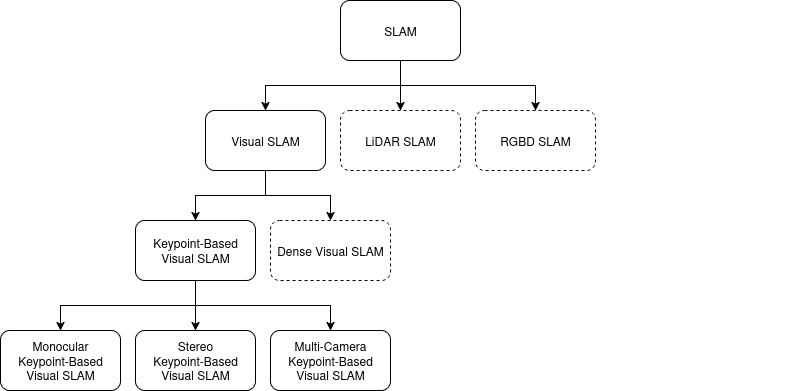
\includegraphics[width=0.8\textwidth]{resources/slam_family_tree.png}
    \caption{Keypoint-based Visual SLM pipeline showing the flow of data from sensor input to map and pose output.}
    \label{fig:slam_family_tree}
\end{figure}

% What is SLAM? What are its goals? What are its use cases?
SLAM refers to the joint problem of simultaneously generating a map of an environment and estimating the position of an observer within that map based on sensor observations. With research beginning in the 1980s \cite{smithEstimatingUncertainSpatial1988}, SLAM has become a de facto standard in robotics for tasks which require operations within unfamiliar environments. The benefit of SLAM when compared to other navigation methods such as pure localization is the ability to operate with no a-prioiri information, instead creating and incrementally updating the map at runtime. The selection of sensors is extremely flexible, with many popular implementations existing for camera, LIDAR, and RGBD based sensor modalities. Through careful selection of sensors, SLAM systems can operate in a wide variety of environments, from indoor office spaces to densely forested areas, and even underwater or in space.  These features make SLAM a powerful too for autonomous navigation, leading to its widespread use in robotics, augmented reality, and autonomous vehicles.

% What are the defining characteristics of keypoint based visual SLAM as opposed to other SLAM methods?
This research targets Keypoint-Based Visual SLAM (KV-SLAM), a specific modality of SLAM characterized by its use of one or more cameras as the primary sensor, and the use of keypoints as opposed to raw pixel values as the primary data for constructing the map and performing localization. As opposed to other sensor modalities such as LIDAR and RGBD, which take direct 3D measurements of the environment, KV-SLAM relies on the principles of epipolar geometry to infer depth and camera motion from the relative position of keypoints between image frames. The map generated by a KV-SLAM system is a sparse point cloud of 3D map points. Core to this research is the concept of the keypoint, map point, and sparse map, motivating a discussion on the definitions and structure of these types, and how they relate to the larger KV-SLAM pipeline.


% Describe the structure of a map in kvSKAM, including keyframes, map points, and their relationships.
The primary input to a KV-SLAM system is the keypoint. A keypoint is the combination of an image feature and a descriptor. Image features can take many forms, but for the purposes of SLAM, they should be identifiable, meaning they are quick to compute, and differentiable, meaning they are unique enough to tell one instance of a feature from another. Image features are differentiated using a descriptor, which is a vector representation of the feature that captures its unique characteristics. Ideally, keypoints should be invariant to changes in scale, rotation, and illumination, allowing them to be reliably matched between images taken from different viewpoints or under different lighting conditions.

Map points represent the extrapolation of keypoints into 3D space. Two views of the same set of keypoints can be used to triangulate the 3D position of the visual feature, in conjunction with the camera transformation between the two views. Depending on the implementation, map points often store additional metadata, such as the set frames in which they were observed, the descriptors of the keypoints they were derived from, etc. The primary contribution of this research is a novel method of determining and representing the observability of map points at the individual point level, allowing for the efficient and accurate identification of outdated map points.

The sparse map is the collection of all map points, acting as a 3D representation of the environment. It is used to localize new frames by finding a transformation that aligns the currently seen keypoints with the existing map points. This 2D-3D alignment is accomplished through an optimization process which iteratively refines the camera transform to minimize the reprojection error between the matched features.

% Explain how data flows through a keypoint-based visual SLAM system, from sensor input to map and pose output.
With these structures in hand, we can describe the pipeline which data follows through a generic KV-SLAM system. A graphical representation of the pipeline can be seen in Figure \ref{fig:kv_slam_pipeline}, each stage is expanded on here.

1. Initialization

\begin{figure}[!ht]
    \centering
    % \includegraphics[width=0.8\textwidth]{figures/kv_slam_pipeline}
    \caption{Keypoint-based Visual SLAM pipeline showing the flow of data from sensor input to map and pose output.}
    \label{fig:kv_slam_pipeline}
\end{figure}

% High level overview of the challenges of SLAM: computational complexity, sensor error accumulation, dynamic environments
This high-level overview of KV-SLAM Despite numerous advancements, the computational complexity of performing SLAM in real-time remains a challenge, meaning that on many resource constrained platforms, implementations can struggle to keep up with the rate of sensor data acquisition \cite{semenovaQuantitativeAnalysisSystem2022}. Additionally, because there is no fixed reference, SLAM systems can suffer from sensor error accumulation, leading to inaccurate maps and poses over time \cite{cadenaPresentFutureSimultaneous2016}. These issues are compounded as the timeframe, scale, and environmental dynamics of the SLAM task increase. Larger environments require larger, more complex maps, which produce higher computational load and longer processing times. Dynamic environments, where objects can move or change either during the SLAM process or between runs, are a particular challenge, as most SLAM systems tend to operate best in static environments, and can struggle to maintain accurate pose estimation and map consistence in the presence of moving objects. The field of SLAM research known as \textit{lifelong SLAM} \cite{cadenaPresentFutureSimultaneous2016} focuses on addressing these challenges, and will be covered in detail in Section \ref{sec:related_work}.


\subsection{ORB-SLAM3}

ORB-SLAM3 is a KV-SLAM implementation which is popular in research contexts due to its performance

\subsubsection{Loop Closure}
\subsubsection{Relocalization}
\subsubsection{Map Reuse}
\subsubsection{Map Point Culling}
\subsection{The Von Mises-Fisher Distribution}

This work uses the von Mises-Fisher distribution, a probability distribution defined on the unit sphere, as the basis for the viewpoint-a

\section{Related Work}
\label{sec:related_work}

This chapter contextualizes this thesis within the broader body of SLAM research. The topics discussed are selected for their relevance to two previously outlined objectives: the identification and removal of data that could cause instability, and the improvement of SLAM performance over long time horizons. While the goals of this research align with the topics of semantic rejection and lifelong SLAM, the methods applied are more closely related to change detection, point stability and re-observability confidence. The following sections explore the key ideas from these topics, and relate them to the proposed research.

\subsection{Change Detection}

In the context of SLAM, change detection refers to the identification of discrepancies between the map and the environment. In lifelong SLAM operations, change detection is often used to assist with map maintenance tasks by identifying areas of change and updating them to match the current environment. However, change detection has been used for many other purposes. Change detection methods can be split based on the abstraction level at which they operate.

\subparagraph{Object Level}
Larsen et al. \cite{larsenChangeDetectionModel} utilized pairs of images to identify geometric inconsistencies in existing 3D maps, allowing for the identification of individual added or removed objects.

\subparagraph{}

\subsection{Lifelong SLAM}

The term Lifelong SLAM has varied definitions throughout the literature, but common themes of robustness to dynamic change, and long-term operation can be seen. For simplicity, this research adopts the definition provided by Shi et al. \cite{shiAreWeReady2020}, describing lifelong SLAM as the ability for a robot to generate, maintain, and localize within a map of a particular environment over an extended period of time. This is in contradistinction to the standard SLAM operating model, which tends to require short timeframes due to the assumption of a static environment. Unlike standard SLAM, lifelong SLAM is expected to operate despite environmental changes such as moved objects, lighting changes, dynamic objects within sensor view, etc. Some topics which fall under the umbrella of lifelong SLAM field have already been discussed, such map reuse. An exploration of previous lifelong SLAM work is provided below, grouped by the specific challenge addressed by the research.

\subsubsection{Place Recognition}

As previously discussed, the ability to recognize previously visited areas allows a SLAM system to perform important operations like relocalization and loop closure, increasing robustness and reducing global map error. Place recognition in standard SLAM is already nontrivial, requiring methods to efficiently identify similarity between historical data and current sensor readings. In lifelong SLAM, the problem becomes more challenging, as relocalization methods must handle the possibility of visual or geometric changes to the environment.

ORB-SLAM3 performs place recognition with a visual bag-of-words approach, producing a hierarchical database of localized frames based on the visual features observed within the frame \cite{camposORBSLAM3AccurateOpenSource2021}\cite{galvez-lopezBagsBinaryWords2012}. This database is queried with visual features observed by the camera, providing candidate positions identified by visual similarity. However, as implemented, ORB-SLAM3's place recognition does not fulfil the objectives of lifelong SLAM. While the system may successfully place recognize despite some dynamic changes, no effort is made to recognize these changes or update internal representations based on observations, leading to failures in dynamic situations.



\subsubsection{Map Reuse}
\subsubsection{Map Maintenance}
\subsubsection{Change Detection}
\subsubsection{Dynamic Object Detection}


\subsection{Change Detection}

Change detection refers to the process of detecting discrepencies between  the detection and identification of 


\section{Implementation}

\subsection{Method Overview}

% This section details the methods researched for modeling historical map point observability, and explores how it may be used to identify outdated map points. The methods explored here will be tested and benchmarked in Section \ref{sec:analysis} to determine if the objectives laid out in Section \ref{sec:objectives} are successfully achieved.

% The objective is to identify map points which, while previously viewed, are no longer visible due to environmental changes. To address this, we assign an incrementally updated probability of existence value to each map point. Observations of a map point increase our overall confidence in its existence. Conversely, failure to observe a map point from a viewpoint where it \textit{should} have been visible lowers our confidence in its existence. Determining whether a map point should be observable from a given viewpoint is not trivial, motivating the need for a viewpoint-aware observability model. The purpose of the model is to integrate historical observability data to estimate observability across all possible viewpoints. Each map point is attached to its own model.

\subsubsection{The Existence Estimation Framework}

The existence estimation framework intends to iteratively update a confidence estimate for each map point in a reused KV-SLAM map using historical observability priors and current observations to accurately update the confidence value. As shown in \ref{fig:existence_estimation_framework}, the framework operates on observational data, and returns an updated estimate of the point's probability of existing.

\begin{figure}[!ht]
    \centering
    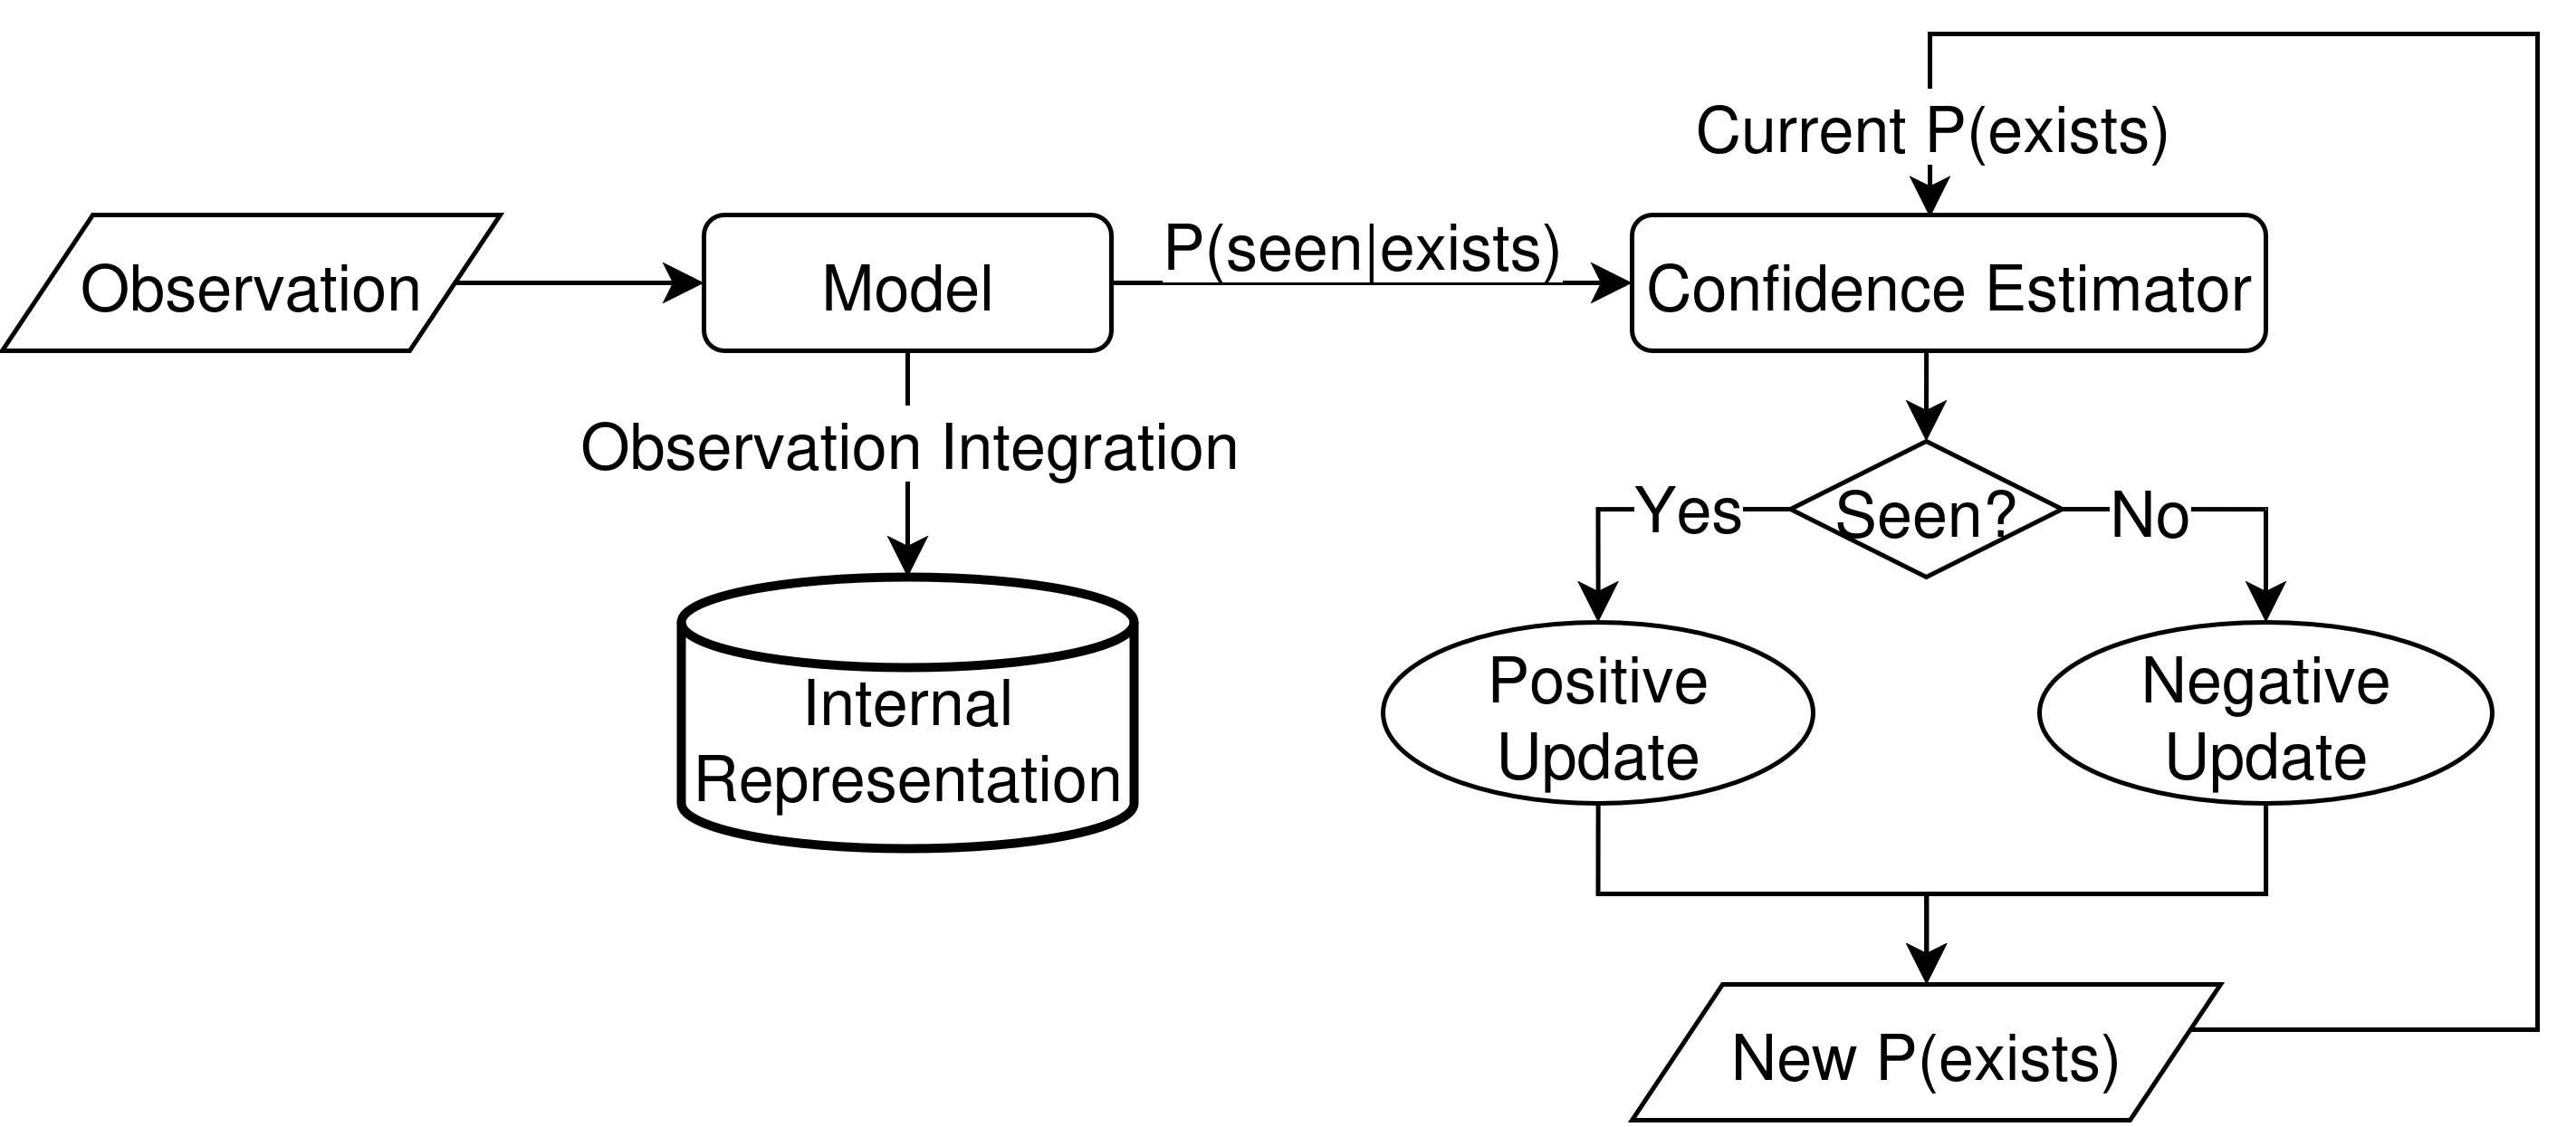
\includegraphics[width=0.7\textwidth]{resources/existence_estimation_framework.png}
    \caption[Existence Estimation Framework]{A flowchart representing the flow of data through the proposed Existence Estimation Framework.}
    \label{fig:existence_estimation_framework}
\end{figure}

The framework contains two core components: the observability model, and the confidence estimator. The observability model is responsible for estimating the probability of the point being seen from a given position, and integrating the new observation into its internal representation of the point's observability. The confidence estimator performs a Bayesian update of the point's probability of existence, utilizing the point's prior existence probability, the estimated likelihood of the point being seen from the model, and whether the observation was successful to generate the new estimate. This combination allows negative observations from viewpoints from which the model believes the point should be observable to impact the overall probability of existence more than observations from lower confidence viewpoints. Additionally, by integrating the new observations into the model, the system effectively prevents repeated observations from the same viewpoint from overly pelanalizing the probability estimate

\subsubsection{The Bayesian Update Step}

The system updates its confidence for a map point's existence based on environmental observations. This update follows Bayes' theorem, and can therefore be implemented to utilize Bayesian statistics. The events of interest are:
\begin{itemize}
    \item $E$: The event that the map point exists
    \item $S^{\boldsymbol{v}}$: The event that the map point is seen from viewpoint $\boldsymbol{v}$
\end{itemize}

where $\boldsymbol{v} = \{\theta,\phi,d\}$, representing azimuth, elevation and distance from the observer to the point respectively. To formalize, our system updates $P(E) = P(E|S^{\boldsymbol{v}})$ given a positive observation, and $P(E) = P(E|\neg S^{\boldsymbol{v}})$ given a negative observation.

Applying Bayes' theorem, the derived update function is
\[
    P(E) = \begin{cases}
        \frac{P(S^{\boldsymbol{v}}|E)P(E)}{P(S^{\boldsymbol{v}})}           & \text{given }S^{\boldsymbol{v}}      \\
        \frac{P(\neg S^{\boldsymbol{v}}|E)P(E)}{P(\neg S^{\boldsymbol{v}})} & \text{given }\neg S^{\boldsymbol{v}}
    \end{cases}
\]

Additionally, the marginal probability $P(S^{\boldsymbol{v}})$ is
$$
    P(S^{\boldsymbol{v}}) = P(S^{\boldsymbol{v}}|E)P(E) + P(S^{\boldsymbol{v}}|\neg E)P(\neg E)
$$

The probability of a false observation of a non-existent map point is small, but non-zero. The probability of a false match increases in low-light and in low texture environments. The value $\varepsilon$ is assigned to represent this probability, and will be experimentally determined in Section \ref{sec:existence_confidence_eval}.
$$
    \varepsilon = P(S^{\boldsymbol{v}}|\neg E) \approx 0
$$

Finally, assuming the existence of a model function $m$ which estimates the probability of observing the point from a given viewpoint $\boldsymbol{v}$
$$
    m(\boldsymbol{v}) \approx P(S^{\boldsymbol{v}}|E)
$$

The update step can be expressed as
\[
    P(E) = \begin{cases}
        \frac{m(\boldsymbol{v})P(E)}{m(\boldsymbol{v})P(E) + \varepsilon(1-P(E))}             & \text{given }S^{\boldsymbol{v}}      \\
        \frac{(1-m(\boldsymbol{v}))P(E)}{(1-m(\boldsymbol{v}))P(E) + (1-\varepsilon)(1-P(E))} & \text{given }\neg S^{\boldsymbol{v}}
    \end{cases}
\]

\subsubsection{The Observability of Map Points}

Map points are conceptualized as static, infinitesimally small points in 3D Euclidean space. Let the observability of a map point $p$ from a viewpoint $\boldsymbol{v} = \{\theta,\phi,d\}\in[0,2\pi)\times\left[-\frac{\pi}{2},\frac{\pi}{2}\right]\times[0,d_{max})$ be represented by the function
$$
    \operatorname{observable}_p : V \to \{0, 1\}
$$
where $\boldsymbol{v} = \{\theta,\phi,d\}$ represents the azimuth, elevation, and distance from the observer to $p$ respectively. This function returns 1 if $p$ is observed from $\boldsymbol{v}$, and 0 if it is not. From this, an observation of point $p$ can be defined as a vector $\boldsymbol{o}_p=\{\boldsymbol{v},observable_p(\boldsymbol{v})\}$, and a set of $n$ observations of $p$ as $\boldsymbol{O}_p=\{\boldsymbol{o}_{p0},\dots,\boldsymbol{o}_{pn}\}$. For illustrative purposes, figures in the remainder of this thesis may use a simplified 2D representation of these definitions, where $\boldsymbol{v}^{2D}=\{\theta,d\}$. Figure \ref{fig:global_observability_p} shows such a plot representing the global observability of a map point $p$, and the effects of obstructions on observability.

\begin{figure}[!ht]
    \centering
    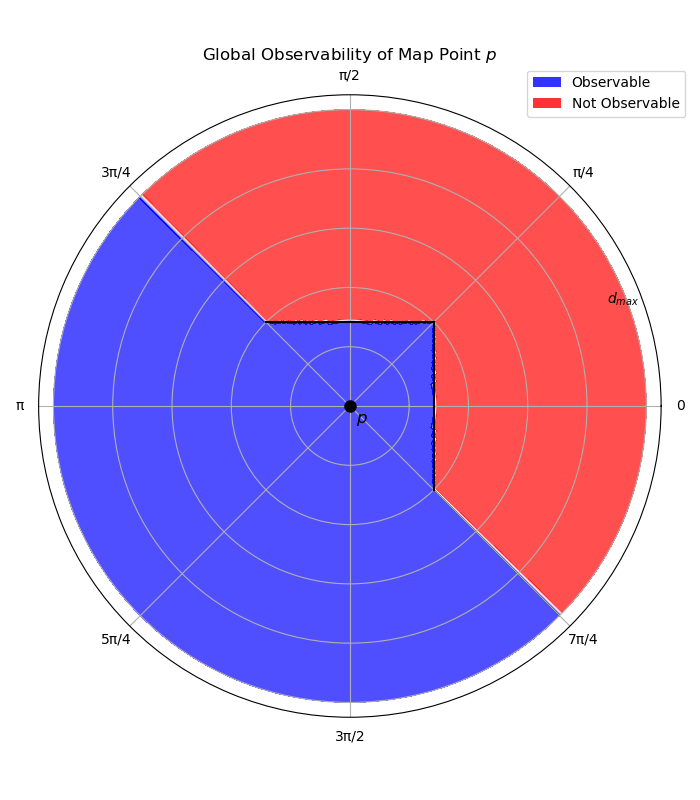
\includegraphics[width=0.7\textwidth]{resources/global_observability_p.png}
    \caption[2D Global Observability]{A 2D representation of the global observability of a map point $p$ near two orthogonal obstructions.}
    \label{fig:global_observability_p}
\end{figure}

It should be noted that within Euclidean space, a map point which is occluded from a viewpoint $\boldsymbol{v} = \{\theta, \phi, d\}$ will also be occluded from any viewpoint $\boldsymbol{v}' = \{\theta, \phi, d'\}$ where $d'>d$. Therefore, any positive observation from a direction which was previously observed to be occluded must be the result of either a false positive, or the removal of the occlusion.

% Therefore, the global observability of a map point can also be represented using the function
% \[
%     \operatorname{barrier}_p : \mathbb{S}^2 \to \mathbb{R}^+, \quad
%     \operatorname{barrier}_p(\boldsymbol{u}) = \argmin_d \operatorname{observable}_p(\boldsymbol{u}, d)
% \]

The left plot of Figure \ref{fig:2d_observability} represents the output of a simplified 2D version of the observability function across the domain of $\theta\times d$, and the effects of obstructions on the observability. However, to generate such a plot from sensor data would require infinite observations spanning the full domain of $\theta\times d$. Instead, the system must operate on a finite set of observations as shown in the plot on the right. As described above, the Bayesian update step requires a model function $m$, the output of which is the probability of observing the point from a given position based on the historical observability of the map point. There are many possible implementations for the model, with the three implementations tested described below.

\subsubsection{Modeling Historical Observability of Map Points}

The goal of the model is to estimate the global observability of a point using a finite set of $n$ observations $\boldsymbol{O} = \{o_0,\dots,o_n\}$, an implementation-dependent set of $k$ model parameters $\boldsymbol{x}=\{x_0,\dots,x_k\}$, and a current viewpoint $\boldsymbol{v}$.
$$
    m(\boldsymbol{O},\boldsymbol{x},\boldsymbol{v})\to[0,1]
$$

Therefore, the model functions will be implemented with the goal of minimizing the objective function
$$
    \iiint |m(\boldsymbol{O},\boldsymbol{x},\boldsymbol{v}) - v(\boldsymbol{v})| \,d\theta\,d\phi\,dd
$$

Additionally, the models are constrained by the goals laid out in Section \ref{sec:objectives} for speed and size of the model. The integrated version which will be described in Section \ref{sec:orb_slam3_integration} must run in real time, meaning inserting new observations should be fast. Additionally, as the model parameters will be stored in memory during operations, and written to disk for map reuse, the additional space required by the model must be minimized. Each of the three models described will be compared for speed, size, and accuracy, and the parameters to each model will be tuned using non-linear optimization to determine the best possible parameterization. With these goals in mind, the model implementations can now be described. These models were selected based on their ease of implementation and simple methodology. This is not the complete set of possible implementations, and are not guaranteed to be the optimal solution to modeling historical map point observability while maximizing accuracy and minimizing time and storage usage.

\paragraph{K-Nearest Neighbors Model}
A simple method for modeling the observability is the use of a K-nearest-neighbors clustering method. The only parameter in such a model. Such a model could be formulated as follows:
$$
    m_{knn}(k, n, \boldsymbol{v}) = \frac{a}{b}
$$
\paragraph{Binned Model}
\paragraph{Continuous Model}

\subsection{Observability Model Implementation}

The implementations explored in this thesis serve as representative examples of various methods for modeling map point observability. While not an exhaustive exploration of all possible methods or implementations, these examples provide a foundation for future research.

Each model described below is initialized with a vector of inputs representing various tunable parameters for the model. The final selection of these inputs will be tuned through an optimization process described in Section \ref{sec:parameter_tuning}. Each model provides functions query and integrat which returns the models estimate of $P(S^{\boldsymbol{v}}|E)$, integrating new observations into the internal representation, and optionally, receiving feedback from the Existence Probability Estimator.

\paragraph{K-Nearest Neighbors Model}

A simple method for modeling the observability is the use of a K-nearest-neighbors clustering method. In this model, the estimation is the number of positive observations in the k-nearest observations divided by k. The replacement strategy utilizes feedback from the existence estimator, replacing the nearest observation with the new observation if $\Delta P(E) > \tau$ where $\tau$ is a threshold found through optimization.

\begin{singlespace}
    \begin{algorithm}[H]
        \caption{KNN Query}
        \label{alg:query}
        \begin{algorithmic}
            \Require Viewpoint $v = (\theta, \phi, d)$
            \Require Previous observations $[(\theta_0, \phi_0, d_0, \text{seen}_0),\dots,(\theta_n, \phi_n, d_n, \text{seen}_n)]$
            \Require Parameters $k$, \texttt{max\_angle}
            \Ensure Estimated probability of seeing the point from $v$

            \State $candidates \gets [\;]$
            \ForAll{$obs \in observations$}
            \State $obs\_view \gets (\theta_i, \phi_i, d_i)$
            \If{$\texttt{angular\_dist}(v, obs\_view) \leq \texttt{max\_angle}$}
            \State $dist \gets \texttt{euclidean\_dist}(v, obs\_view)$
            \State $candidates.\texttt{append}((dist, obs))$
            \EndIf
            \EndFor
            \State Sort $candidates$ by $dist$ in ascending order
            \State $k\_neighbors \gets$ first $\min(k, \texttt{length}(candidates))$ entries
            \If{$\texttt{length}(k\_neighbors) = 0$}
            \State \Return $0.5$
            \EndIf
            \State $n\_seen \gets$ count of entries in $k\_neighbors$ where $\text{seen} = \text{True}$
            \State \Return $n\_seen / \texttt{length}(k\_neighbors)$
        \end{algorithmic}
    \end{algorithm}
\end{singlespace}

Parameters to Optimize: $[n, k, \tau]$

\paragraph{Binned Model}

In this model, each observation is assigned to a bin based on the unit direction of observation. Each bin stores the maximum distance from which it was observed, total number of observations within that distance, and the number of positive observations within that distance. The estimate is the number of positive observations within the distance divided by the total number of observations, or 0 if the observation occurs outside the observability shell.

\paragraph{Continuous Model}

\subsubsection{Icosahedral Shell Implementation}
\label{sec:icos_construction}

\subsection{Bayesian Update Implementation}

\subsection{Existence Estimation Framework Implementation}

\subsection{ORB-SLAM3 Integration}

\subsection{Dataset Creation}

\subsection{Experimentation Setup}


\section{Experimental Analysis}

\label{sec:}

\subsection{Evaluation Metrics}
\label{sec:eval_metrics}

\subsection{SLAM System Configurations}

\subsubsection{Parameter Tuning}

\subsection{Results}

\subsubsection{Quantitative Evaluation}

\subsubsection{Qualitative Evaluation}

\subsubsection{Ablation Study}


\section{Discussion}


\section{Conclusion and Future Work}


\addcontentsline{toc}{section}{References}
\printbibliography

\section*{Appendices}
\addcontentsline{toc}{section}{Appendices}

\subsection*{Algorithm Implementations}
\addcontentsline{toc}{subsection}{Algorithm Implementations}

\subsection*{Full Results}
\addcontentsline{toc}{subsection}{Full Results}

\end{document}